\section{Используемые технологии}

В данном разделе приведено описание языков программирования, фреймворков,
используемых при разработке.

\subsection{Язык программирования \kt{}}
\label{sec:kotlin}

\kt{} (Котлин) --- статически типизированный язык программирования, работающий поверх 
JVM и разрабатываемый компанией JetBrains [2].

Основные приемущества языка \kt{}:
\begin{itemize}
  \item краткость --- кострукции и возможности языка разрабатывались с целью уменьшить 
  количество кода, но при этом не уменьшая читаемости этого кода [3];
  \item поддержка защиты от NullPointerException на уровне языка [3];
  \item полная совместимость с языком программирования Java, что позволяет использовать
  весь набор библиотек и технологий, накопленных за долгое время существования Java;
  \item возможность расширять библиотеки, не изменяя их код, что позволяет дописывать необходимую 
  функциональность без нарушений каких-либо лицензий либо поиска исходников уже 
  скомпилированных библиотек (листинг \ref{lst:kt_ext});
  \item мультипарадигмость --- \kt{} можно писать код как в процедурном стиле, так и в 
  объектно-ориентированном, а также благодаря поддержке функций высшего порядка можно 
  писать код и в функциональном стиле. Сочетание лучших качеств у каждого из этих стилей 
  позволяет разрабатывать приложения быстро и эффективно (листинг \ref{lst:kt_map});
\end{itemize} 

\begin{lstlisting}[style = ktstyle, 
           caption = {Пример Extension-функции на языке \kt{}},
           label = {lst:kt_ext}]
public fun CharSequence.padEnd(length: Int, padChar: Char = ' '): CharSequence {
    if (length < 0)
        throw IllegalArgumentException("Desired length $length is less than zero.")
    if (length <= this.length)
        return this.subSequence(0, this.length)

    val sb = StringBuilder(length)
    sb.append(this)
    for (i in 1..(length - this.length))
        sb.append(padChar)
    return sb
}
\end{lstlisting}

\begin{lstlisting}[style = ktstyle, 
           caption = {Реализация популярной функции высшего порядка <<map>> на языке \kt{}},
           label = {lst:kt_map}]
fun <T, R> List<T>.map(transform: (T) -> R): List<R> {
    val result = arrayListOf<R>()
    for (item in this)
        result.add(transform(item))
    return result
}
\end{lstlisting}

\subsection{Spring Framework}
\label{sec:spring}

Spring --- универсальный фреймворк с открытым исходным кодом для Java-платформы. 
Spring представляет собой набор из большого количества модулей и расширений, позволяющих
эффективно и быстро разрабатывать приложения. Приемущественно он связан с платформой 
Java Enterprise [4].

Spring может быть рассмотрен как коллекция меньших фреймворков. Большинство этих фреймворков 
может работать независимо друг от друга, однако они обеспечивают большую функциональность при 
совместном их использовании. Можно выделить следующие фреймворки, которые делятся на структурные 
элементы типовых комплексных приложений: 
\begin{itemize}
  \item Inversion of Control-контейнер --- конфигурирование компонентов приложений и управление 
  жизненным циклом Java-объектов, поддержка JSR-299 [4];
  \item фреймворк аспектно-ориентированного программирования (AOP) --- работает с функциональностью, 
  которая не может быть реализована возможностями объектно-ориентированного программирования на 
  Java без потерь;
  \item фреймворк доступа к данным: работает с системами управления реляционными базами данных на 
  Java-платформе, используя JDBC- и ORM-средства и обеспечивая решения задач, которые повторяются 
  в большом числе Java-based environments, обеспечивает поддержку Java Persistence API (JPA);
  \item фреймворк управления транзакциями: координация различных API управления транзакциями и 
  инструментарий настраиваемого управления транзакциями для объектов Java [5];
  \item фреймворк MVC: каркас, основанный на HTTP и сервлетах, предоставляющий множество 
  возможностей для расширения и настройки;
  \item фреймворк аутентификации и авторизации: конфигурируемый инструментарий процессов аутентификации и 
  авторизации, поддерживающий много популярных и ставших индустриальными стандартами протоколов, 
  инструментов, практик через дочерний проект Spring Security [5].
\end{itemize}

В данном курсовом проекте задействованы следующие модули Spring:
\begin{itemize}
  \item Spring Boot --- проект для автоконфигурации и работы с другими модулями самого Spring;
  \item Spring Core --- базовый модуль, включающий в себя IoC-контейнер;
  \item Spring MVC --- требуется для быстрой и качественной реализации REST API;
  \item Spring Security --- обеспечивает защиту ресурсов сервера для неавторизованных пользователей, а также
  авторизация по протоколу OAuth 2.0.
\end{itemize}

\subsection{AngularJS}
\label{sec:angular}

AngularJS --- JavaScript-фреймворк с открытым исходным кодом. Предназначен для разработки одностраничных приложений. 
Его цель --- расширение браузерных приложений на основе MVC-шаблона, а также упрощение тестирования и разработки [6].

Фреймворк работает с HTML, содержащим дополнительные пользовательские атрибуты, которые описываются директивами, 
и связывает ввод или вывод области страницы с моделью, представляющей собой обычные переменные JavaScript. 
Значения этих переменных задаются вручную или извлекаются из статических или динамических JSON-данных.

Angular придерживается MVC-шаблона проектирования и поощряет слабую связь между представлением, данными и логикой 
компонентов. Используя внедрение зависимости, Angular переносит на клиентскую сторону такие классические серверные 
службы, как видозависимые контроллеры. Следовательно, уменьшается нагрузка на сервер и веб-приложение становится легче. 
Арихитектура клиентского приложения с использованием AngularJS представлена на рисунке \ref{fig:angular}

Благодаря популярности данного фреймворка существует большое количество пользовательских библиотек (2084, по информации с 
сайта \\ http://ngmodules.org/), которые позволяют ускорить разработку приложения и расширить его функциональность.

\clearpage

\begin{figure}[h!] 
  \centering  
  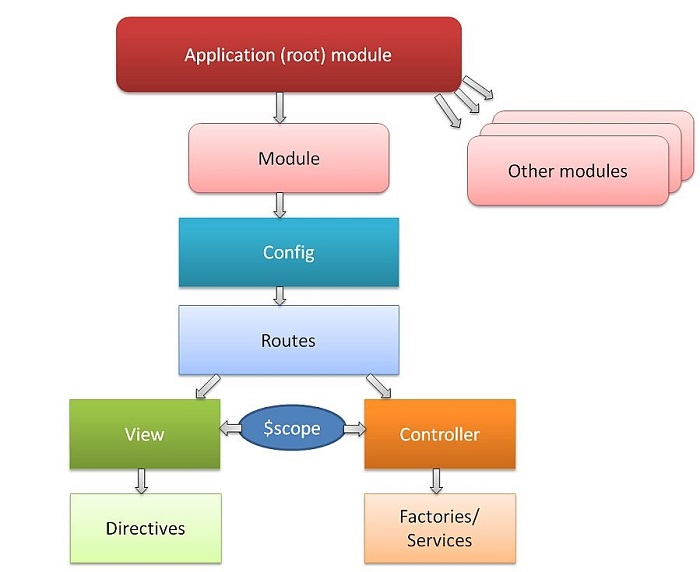
\includegraphics[, scale = 0.65]{angular.jpg}
  \caption{Архитектура приложения с ипользованием AngularJS}
  \label{fig:angular}
\end{figure}